\subsubsection{Amigo}
O projeto Amigo (\emph{Ambient Intelligence for the Networked home environment}) desenvolveu um \emph{middleware} com arquitetura baseada em SOA que integra dinamicamente sistemas heterogêneos para alcançar a interoperabilidade entre serviços e dispositivos. O \emph{middleware} provê a semântica para comunicação e descoberta de dispositivos e serviços disponíveis no ambiente, incluindo dispositivos que utilizam padrões para descoberta como o UPnP integrando dispositivos móveis, computadores pessoais, eletrodomésticos e dispositivos de automação residencial~\cite{amigoArch}.

\begin{figure}[ht]
\center
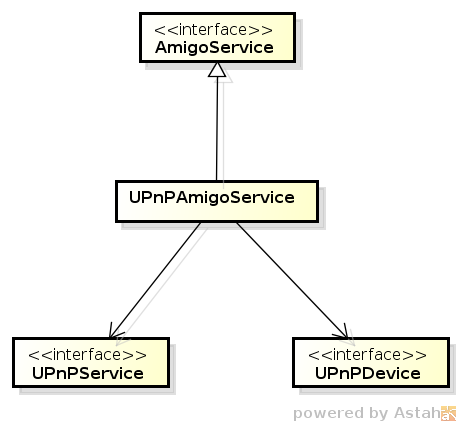
\includegraphics[scale=0.5]{imagens/amigo-interfaces}
\caption{Implementação de um \emph{AmigoService} utilizando serviços UPnP~\cite{amigoCore}}
\label{fig:amigoInterfaces}
\end{figure}

Além de utilizar o UPnP para a descoberta de dispositivos, o Amigo é compatível com as classificações de dispositivos do UPnP. Quando um dispositivo UPnP é encontrado, é criada uma instância de um \emph{UPnPDevice} e o \emph{driver AmigoUPnP} é notificado e executa o método \emph{getServices} do \emph{UPnPDevice} e cria para cada serviço uma instância do \emph{UPnPAmigoService}. A figura~\ref{fig:amigoInterfaces} mostra o relacionamento entre as interfaces UPnP com a implementação de uma interface de um Serviço do Amigo.

Os serviços do Amigo são modelados em uma Ontologia que é utilizada para comparar serviços e decidir se eles são equivalentes. A classe central da Ontologia é o Componente que representa o dispositivo provê o serviço. Para representar o que o dispositivo requer e provê, foi introduzido o conceito da Capacidade, dividida em Capacidade Requerida e Capacidade Provida. Uma Capacidade possui parâmetros de entrada e saída que também são modelados em classes. As capacidades são então associadas à Conversas suportadas pelo Componente e relacionadas à mensagens que são empregadas na Conversa associada como mostra a figura ~\ref{fig:amigoServiceOntology}.

\begin{figure}[ht]
\center
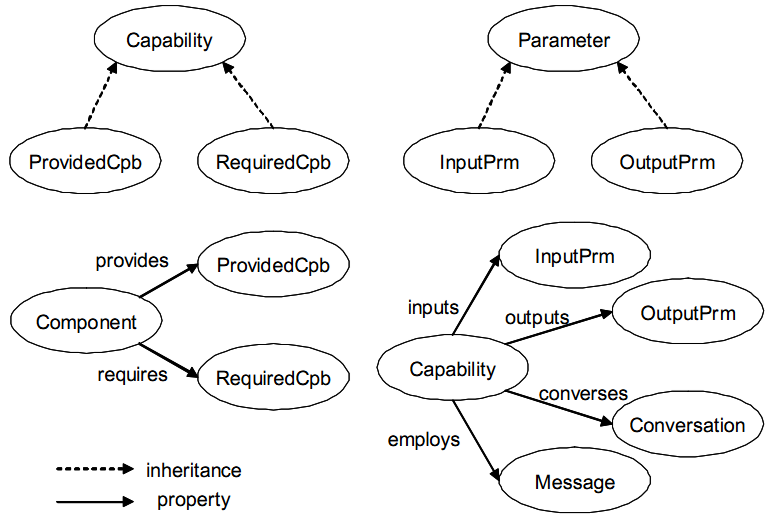
\includegraphics[scale=0.5]{imagens/amigo-ontology}
\caption{Elementos básicos da Ontologia de Serviços~\cite{amigoCore}}
\label{fig:amigoServiceOntology}
\end{figure}


\begin{comment}
http://www.hitech-projects.com/euprojects/amigo/publications/IST-004182%20Amigo-IP%20short%20project%20description.pdf
http://www.hitech-projects.com/euprojects/amigo/deliverables/Deliverable%20D1.2-VolII_SOTA_v10_final.pdf
http://www.hitech-projects.com/euprojects/amigo/deliverables/Amigo_WP2_D2.1_v10%20final.pdf
http://www.hitech-projects.com/euprojects/amigo/deliverables/Amigo_WP3_D31b_v1.0.pdf
\end{comment}
